\documentclass{article}

% Packages
\usepackage[utf8]{inputenc} % UTF-8 input encoding
\usepackage[T1]{fontenc} % Font encoding
\usepackage{amsmath, amssymb} % Math packages
\usepackage{enumitem} % For customizing lists
\usepackage{lipsum} % For generating dummy text
\usepackage{listings}
\usepackage{graphicx}


\lstset{%
  language=bash,
  basicstyle=\fontfamily{pcr}\selectfont,
  commentstyle=\bfseries,
  escapeinside={(*@}{@*)}
}

\newcommand{\comment}[1]{\# here is a comment: #1}
\newcommand\floor[1]{\lfloor#1\rfloor}
\newcommand\ceil[1]{\lceil#1\rceil}

% Title and author information
\title{Algorithms (6470) HW05}
\author{Alex Darwiche}
\date{\today}

\begin{document}

\maketitle

\section*{Answers}

% Question 1
\subsection*{Q1}
\begin{enumerate}[label=(\alph*)]
    \item Prove that if a sequence of relaxation steps ever sets $s.\pi$ to non-NIL value, then G contains a negative weight cycle.
    \item The distance at the source node is 0, so s.d = 0.
    \item For relaxation to ever make it back to s and change its $\pi$, there would need to be a vertex u, such that 0 > u.d + w(u,v).
    \item For this to be true, the distance at vertex u or the edge from u must be negative.
    \item This would mean that there is a negative weight cycle, as s.d would be going below 0.

\end{enumerate}

% Question 2
\subsection*{Q2}
\begin{enumerate}[label=(\alph*)]
    \item Graph G - Bellman Ford Algorithm Results
    \subitem 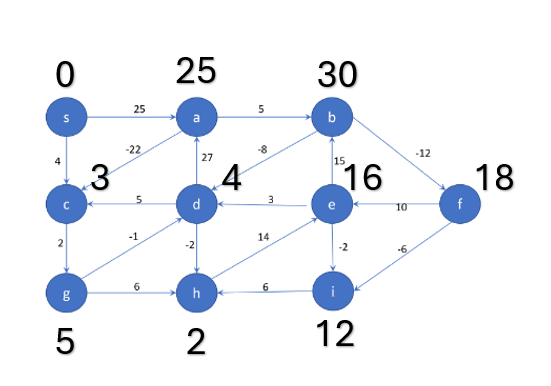
\includegraphics[width=.75\textwidth]{problem2.png}
\end{enumerate}

% Question 3
\subsection*{Q3}
\begin{enumerate}[label=(\alph*)]
    \item Order of Addition of Vertices to Stack: S, A, C, C(lower cost), D, B, B(lower cost), F 
    \subitem 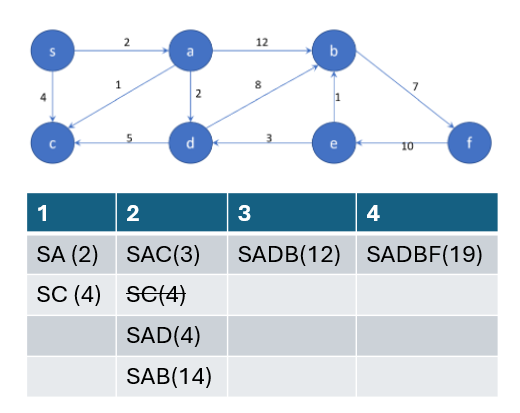
\includegraphics[width=.75\textwidth]{problem3.png} 
\end{enumerate}

% Question 4
\subsection*{Q4}
\begin{enumerate}[label=(\alph*)]
    \item Solving System of Difference Constraints
    \subitem 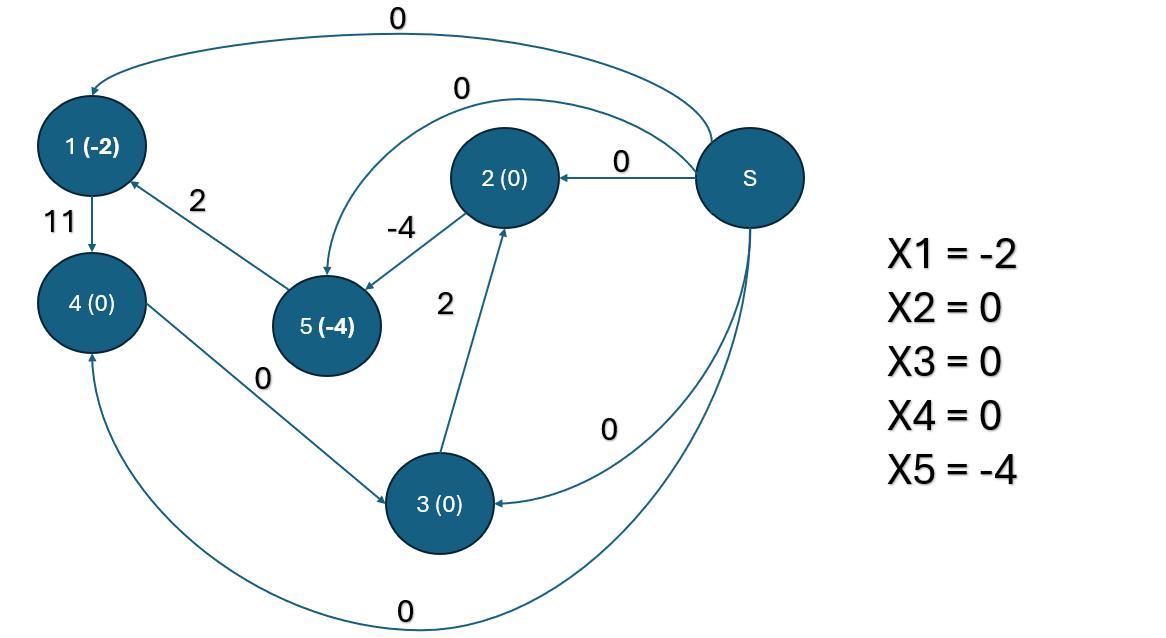
\includegraphics[width=.75\textwidth]{problem4.png}
\end{enumerate}

% Question 5
\subsection*{Q5}
\begin{enumerate}[label=(\alph*)]
    \item Prove that EXTEND is associative. Essentially show that if EXTEND(EXTEND(A,B),C) = EXTEND(A,EXTEND(B,C)).
    \subitem (1) We will start by computing the left and right sides of the above equation with the given information.
    \subitem (2) EXTEND(EXTEND(A,B),C) = $min(min(a_{ij}+b_{jk}) + c_{ij})$
    \subitem (3) $min(a_{ij}) + min(b_{jk}) + min(c_{ij})$
    \subitem (4) EXTEND(A, EXTEND(B,C)) = $min(a_{ij}+ min(b_{ij} + c_{jk}))$
    \subitem (5) $min(a_{ij}) + min(b_{ij}) + min(c_{jk})$
    \subitem (6) As we can see, these expressions are equivalent and thus proves the associativity of the EXTEND algorithm.
 \end{enumerate}

% Question 6
\subsection*{Q6}
\begin{enumerate}[label=(\alph*)]
    \item Residual Chart
    \subitem 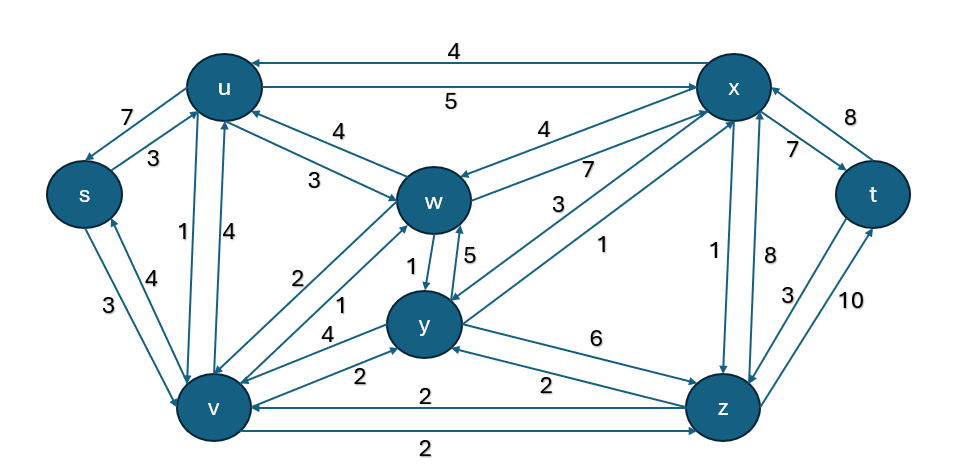
\includegraphics[width=.75\textwidth]{problem6residual.png}
    \item Augmenting path that reduces flow on one edge, increases on others.
    \subitem 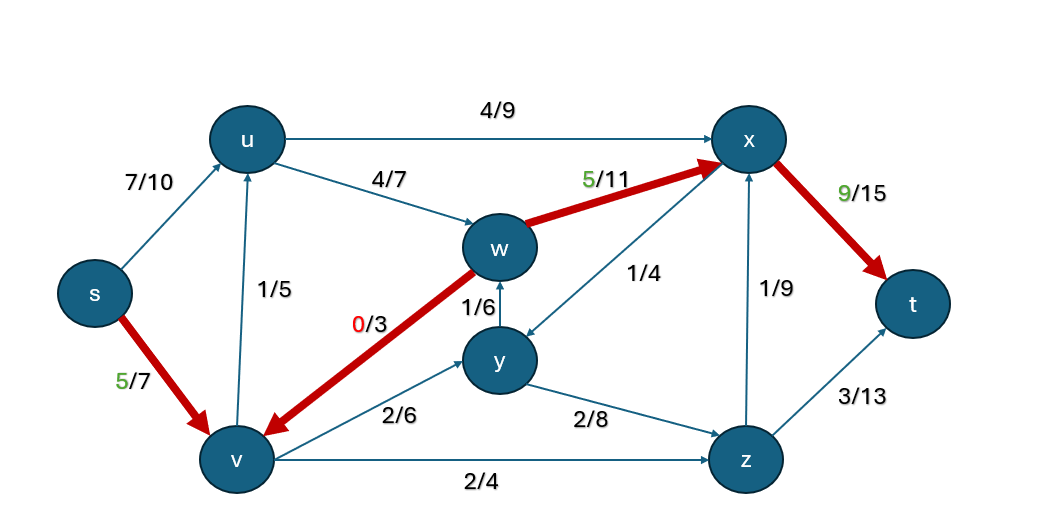
\includegraphics[width=.75\textwidth]{problem6b.png}
    \item (s,v,w,x,t). The flow that goes through this path is 1.
    \item See above for new net flow chart.
\end{enumerate}

% Question 7
\subsection*{Q7}
\begin{enumerate}[label=(\alph*)]
    \item $f(S,T) = 3+2+6-2-0-0 = 9$
    \item $c(S,T) = 15+6+15 = 36$
    \item The following is the min-cut and max-flow of Graph G.
    \subitem 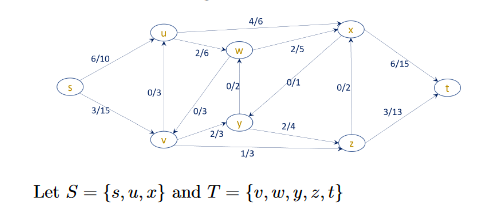
\includegraphics[width=.75\textwidth]{problem7.png}
    \subitem 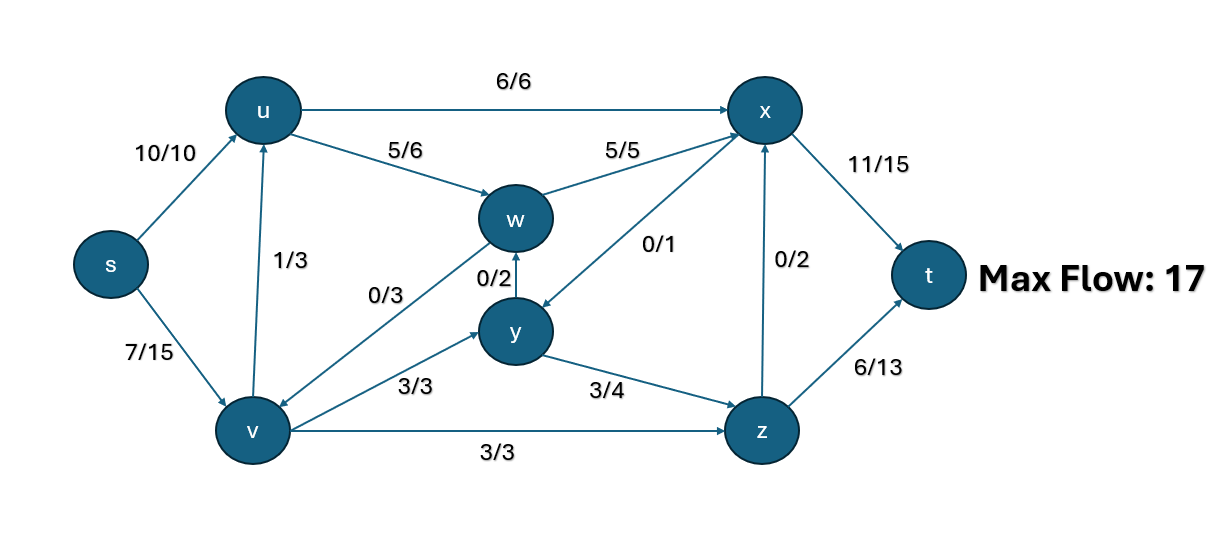
\includegraphics[width=.75\textwidth]{problem7ff.png}
    \subitem 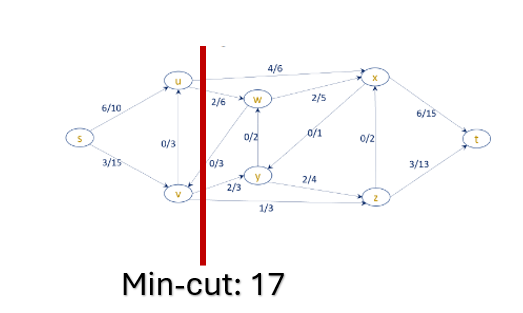
\includegraphics[width=.75\textwidth]{min-cut.png}

\end{enumerate}


% Question 8
\subsection*{Q8     }
\begin{enumerate}[label=(\alph*)]
    \item Johnson's Algorithm, combining Bellman-Ford and Djikstra's Algorithm.
    \subitem 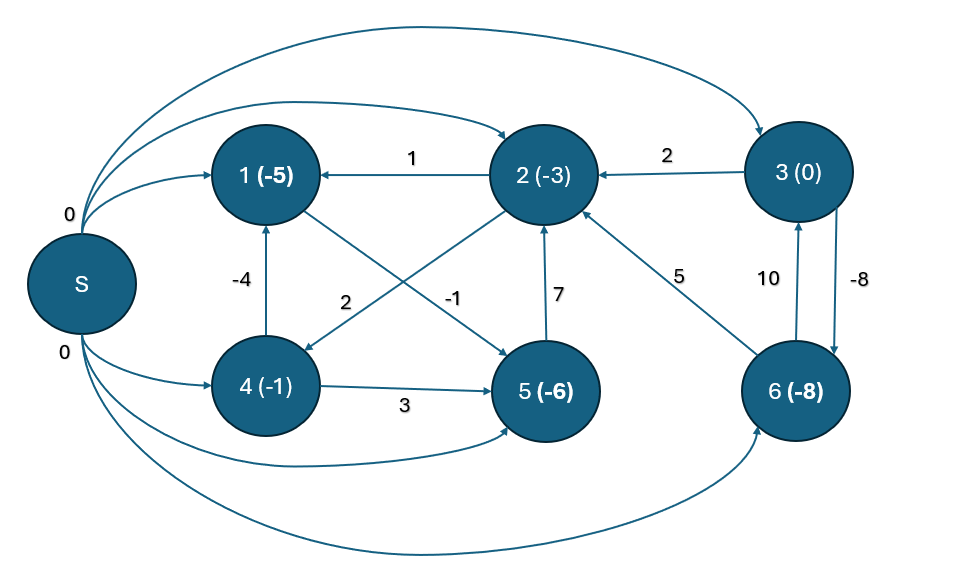
\includegraphics[width=.75\textwidth]{problem8.1.png}
    \subitem 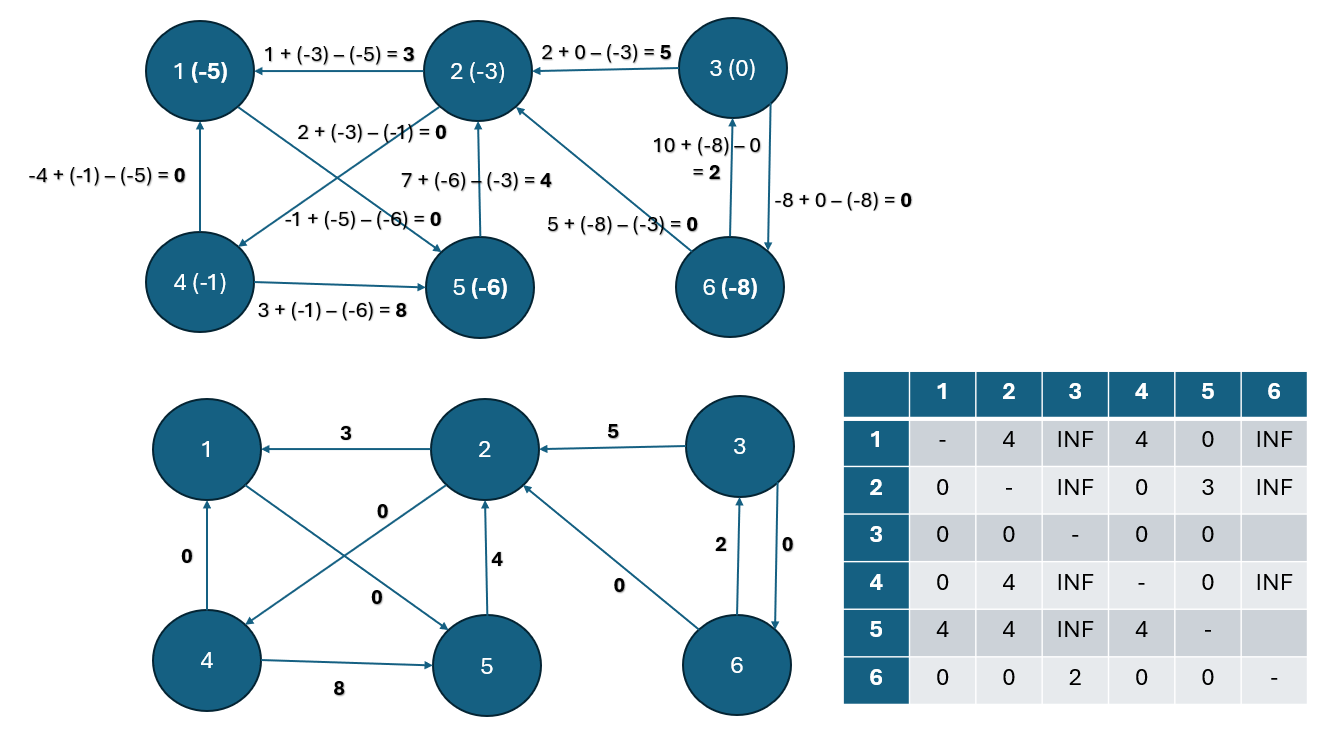
\includegraphics[width=.75\textwidth]{problem8.2.png}

\end{enumerate}

% Question 9 (Graduate students only)
\subsection*{Q1 (Graduate students only)}
\begin{enumerate}[label=(\alph*)]
    \item Psuedocode to count all paths. Basically we're running a DFS style search from each vertex in the graph, and counting each time we hit the goal vertex. This works as each branch of the DFS is a unique path with a distinct start point. To start the DFS from different vertices each time, we will simply reorder the adjaceny matrix each time, until all vertices have been the starting node.
    \begin{lstlisting}[frame=single]
        def COUNT-PATHS(Graph G, Vertex v):
        
        for vertex in G.V:
            \\ We will want to complete a DFS
            \\ for all vertices, and count each
            \\ time they end in the target Vertex v.
            G = reorder-adjaceny(G)
            path_count = DFS(G)

        def DFS(G,v)
            for each vertex in G.V:
                count += DFS-visit(G,vertex,count)
            return count
        
        def DFS-visit(G,v,count)
            for each vertex in G.Adj[u]
                if vertex != v:
                    DFS-visit(G,vertex,count)
                else:
                    count = count + 1
            return count
        \end{lstlisting}
        \item We also do not care about going over a path that has already been gone over, so the coloring shouldn't matter in this algorithm. We are simply looking to extend each neighbor of each child node until it reaches the goal node.
\end{enumerate}

% Question 10 (Graduate students only)
\subsection*{Q2 (Graduate students only)}
\begin{enumerate}[label=(\alph*)]
    \item The following chart shows when Djikstra's algorithm will not work with negative edge weights. You can see that the goal state is achieved while all the AB(10) is still in the stack. This remains in the stack, unexplored, because its value is higher than the goal state. Djikstra's Algorithm makes the assumption that the goal node is reached when the lowest possible path to expand is includes the finishing node. You can clearly see that the shortest path actually involves going from B to C, but this algorithm will not explore that.
    \subitem 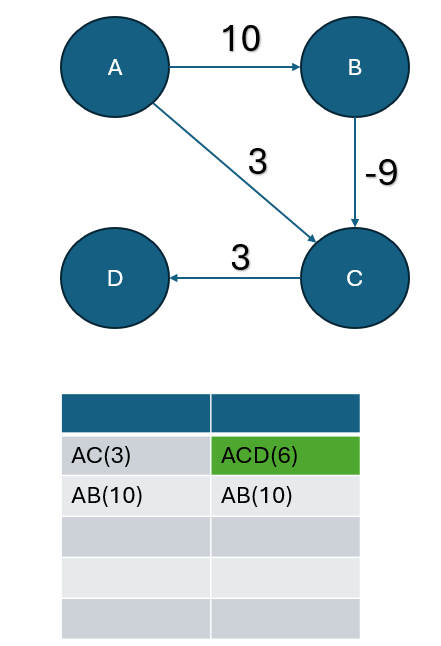
\includegraphics[width=.75\textwidth]{problemg2.png}
\end{enumerate}


\end{document}
